\documentclass[10pt,twocolumn,letterpaper]{article}
\usepackage[T1]{fontenc}
\usepackage[review]{cvpr}
\usepackage{graphicx,amsmath,amssymb,booktabs,microtype,multirow}
\usepackage[pagebackref,breaklinks,colorlinks,allcolors=black]{hyperref}
\def\confName{CVPR}\def\confYear{2027}
\newcommand{\R}{\mathbb{R}}
\newcommand{\E}{\mathbb{E}}
\newcommand{\Var}{\operatorname{Var}}
\newcommand{\InitialError}{0.0578}
\newcommand{\ActiveError}{0.0340}
\newcommand{\FixedError}{0.0423}
\newcommand{\FixedViewError}{0.0403}
\newcommand{\CampaignStatus}{}

\title{Seeing Motion Is Not Identifying Mechanics:\\Joint Material--Interaction Inference with Marginalized Loads}
\author{Anonymous manuscript}
\setlength{\textfloatsep}{8pt plus 1pt minus 1pt}
\setlength{\dbltextfloatsep}{8pt plus 1pt minus 1pt}
\setlength{\floatsep}{6pt plus 1pt minus 1pt}
\begin{document}
\raggedbottom
\twocolumn[{
\renewcommand{\twocolumn}[1][]{#1}
\maketitle
\begin{center}
\IfFileExists{figures/ambiguity.pdf}{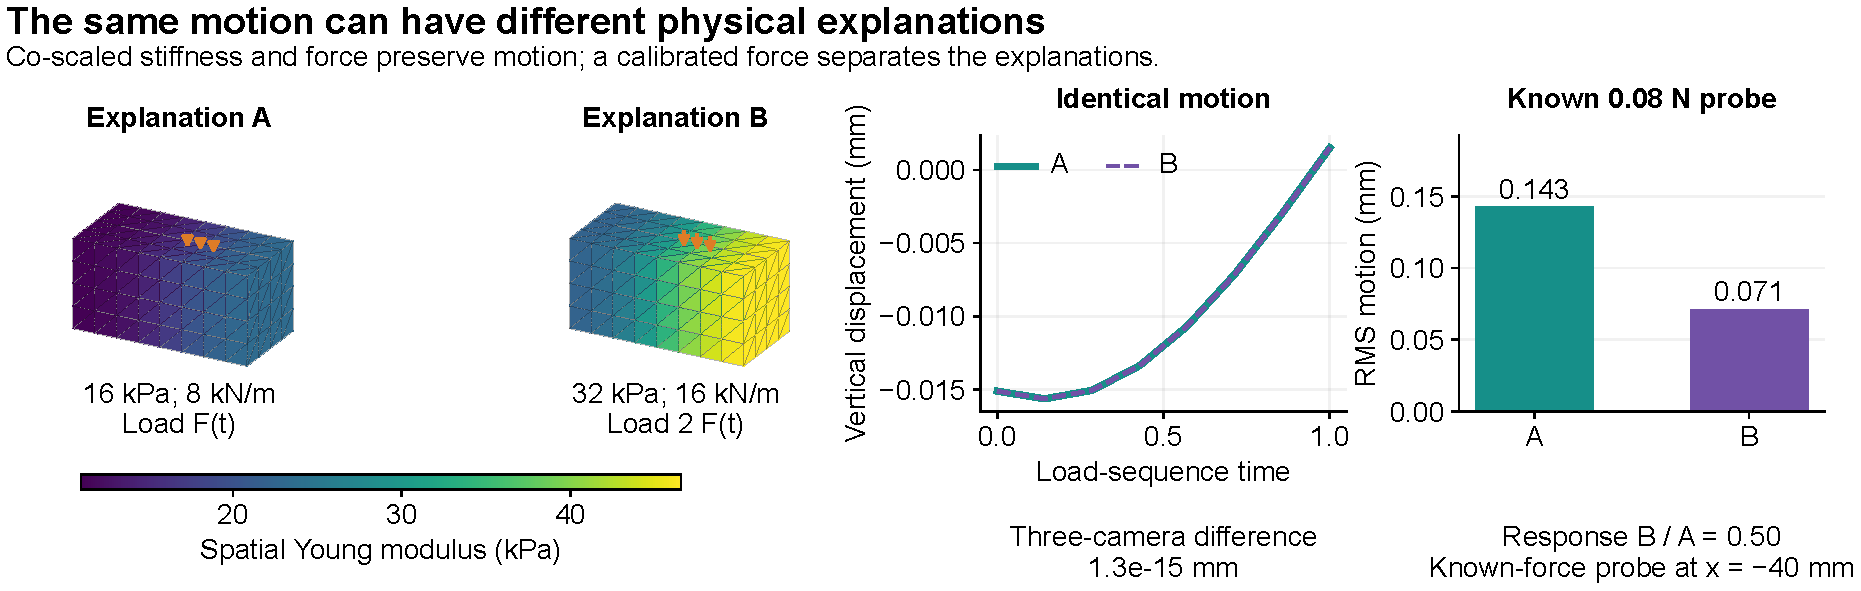
\includegraphics[width=.98\textwidth]{figures/ambiguity.pdf}}{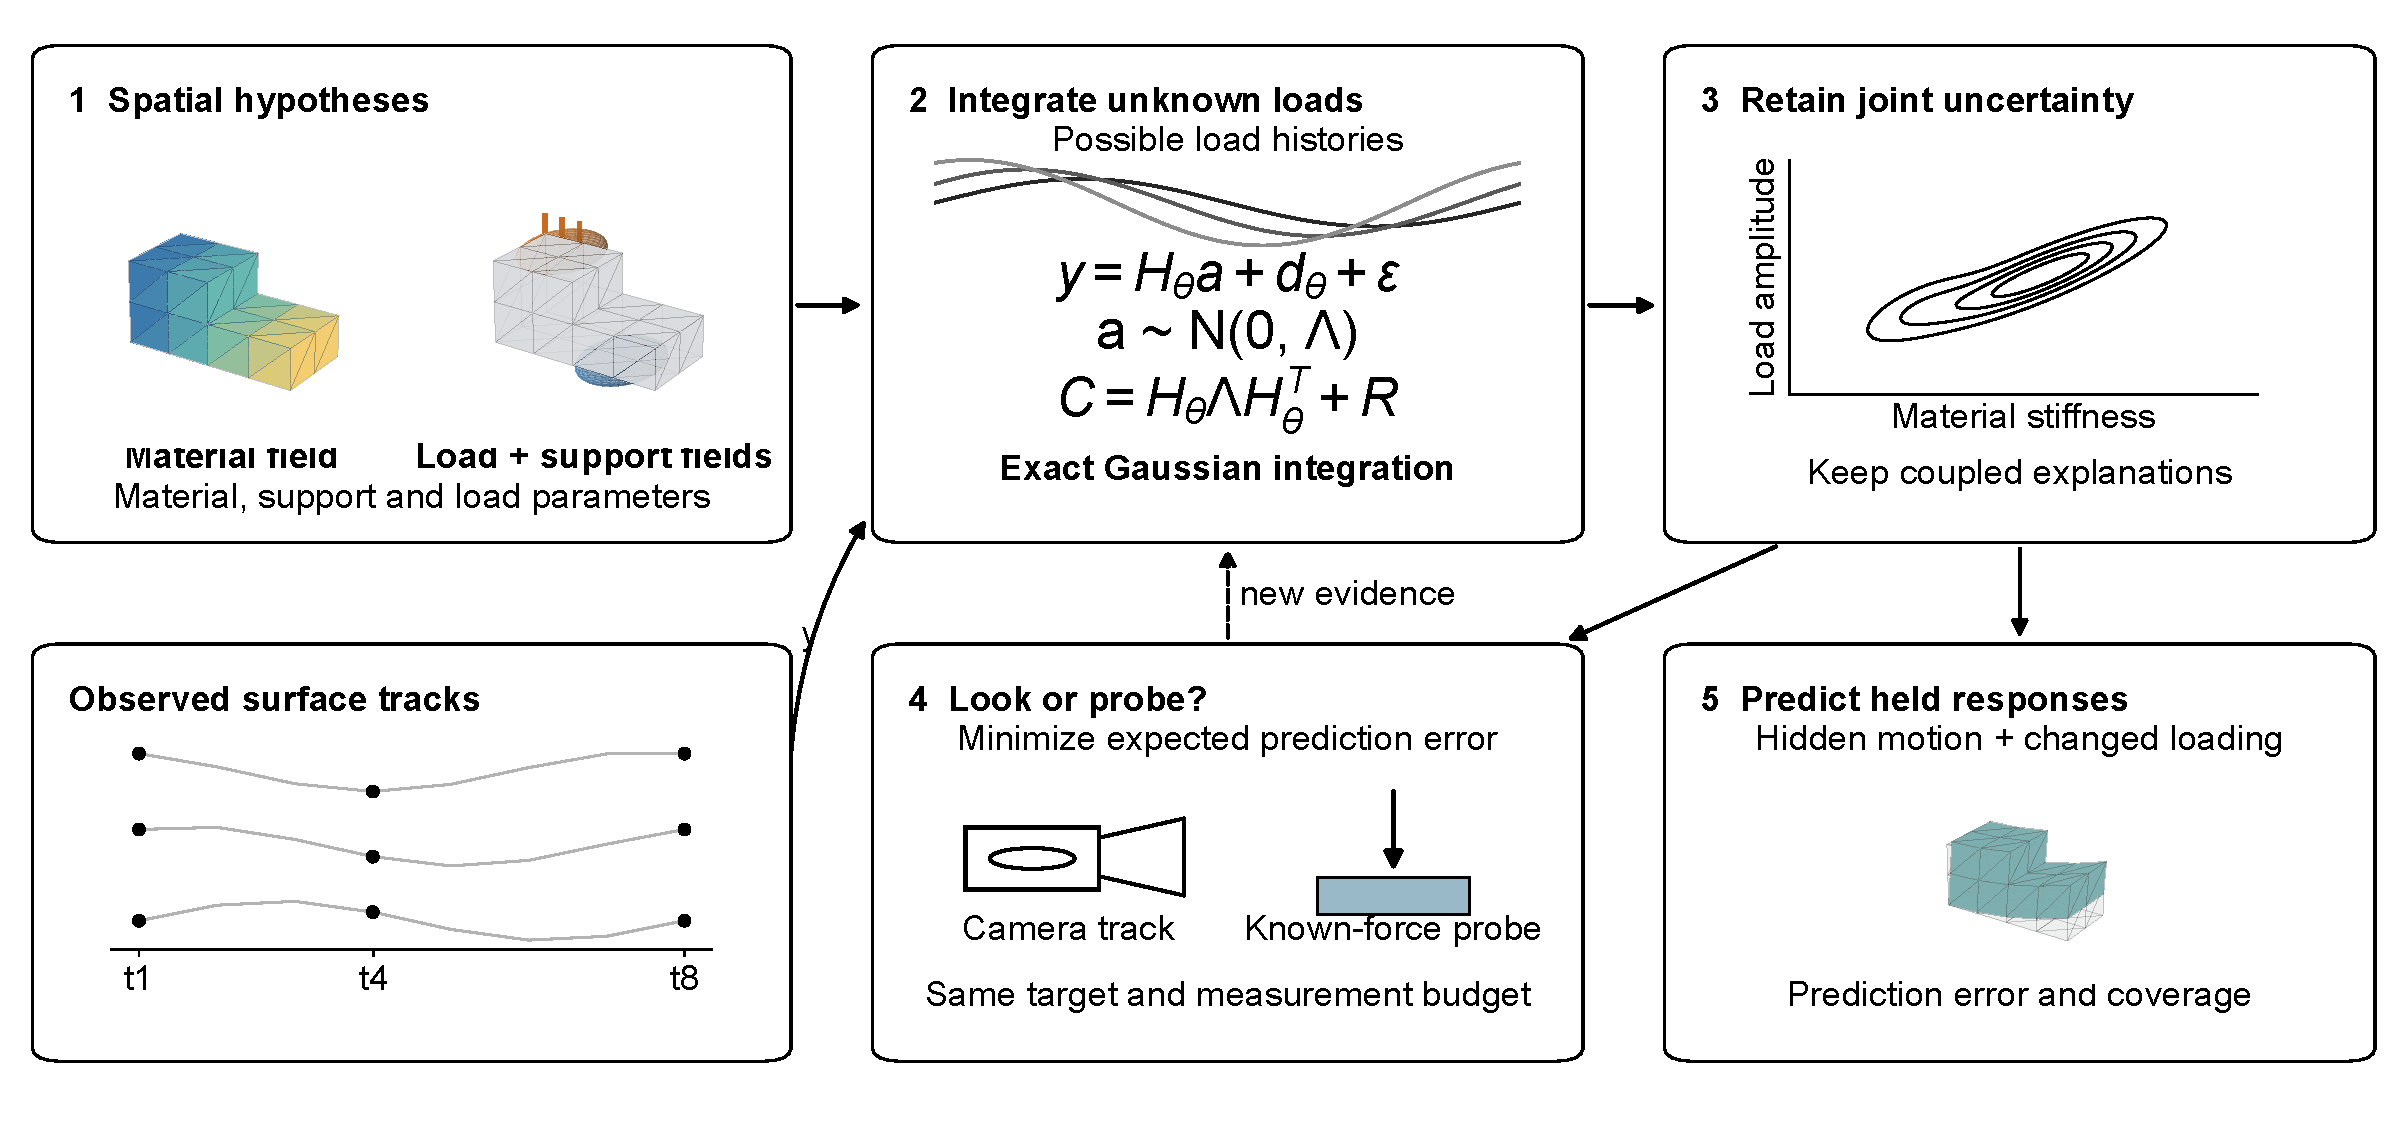
\includegraphics[width=.98\textwidth]{figures/method.pdf}}
\captionof{figure}{\textbf{Identical motion need not imply identical physics.} Scaling elastic stiffness, support stiffness and unknown loads together preserves the observed displacement. A calibrated load does not share that scaling and can distinguish the explanations. Color denotes modulus; bars report volume-weighted nodal RMS. Both explanations lie in the declared dictionary. This constructed symmetry illustrates the identification problem; it is not an inferred posterior or selected benchmark success.}
\label{fig:teaser}
\end{center}
}]
\begin{abstract}
A reconstruction can explain observed motion without identifying how an object will respond to a different interaction. We study this distinction through joint uncertainty over spatial material, support and load fields. Material-attached Gaussian features describe heterogeneous elasticity; separate surface-normalized Gaussian footprints describe compliant support and applied traction. Conditional on these nonlinear field parameters, uncertain temporal load amplitudes are integrated analytically. The posterior retains material--force dependence and compares additional camera tracks with calibrated mechanical probes under one predictive-risk objective. We develop an exact finite-hypothesis reference and continuous sequential Monte Carlo inference, evaluated through known-geometry 3D small-strain mechanics and sparse visible-surface tracks. Across 128 matched cases, four adaptive measurements change coordinate prediction error from \InitialError\ to \ActiveError\,mm; development-selected fixed camera-only and mixed schedules give \FixedViewError\ and \FixedError\,mm. A further 128-case study with uncertain force scale shows that calibrated probes reduce new-load prediction error by 48.4\%, while additional views reduce hidden-motion error by 33.4\%. Continuous-parameter, mesh and force-prior stress tests expose the limits of uncertainty calibration. The results establish a controlled identification and evidence-selection system, with geometry and correspondences supplied, rather than treating visual agreement as proof of physical accuracy. \CampaignStatus
\end{abstract}

\section{Introduction}
A visually convincing deformable reconstruction answers where visible surfaces moved. A physical explanation must additionally say what resists deformation, where constraints act, and which external loads produced the motion. These questions are coupled: increasing material stiffness and applied force can preserve an observed displacement, while changing a support can compensate for a different load footprint. A fitted explanation can therefore interpolate observations yet respond incorrectly to a new intervention.

Recent visual physical twins combine Gaussian appearance with spring or continuum mechanics and demonstrate future motion and changed interactions~\cite{zhong2024springgaus,jiang2025phystwin,xie2024physgaussian}. Learned constitutive models broaden the represented material family~\cite{zhao2025masiv}. Those capabilities motivate a complementary question: \emph{which aspects of the inferred explanation are determined by the available evidence, and which additional measurement improves a specified physical prediction?} More expressive mechanics alone does not answer it. An unknown force can compensate for a material error; a narrow conditional force interval can hide uncertainty in the material to which it is conditioned.

We investigate a tractable joint identification model. Spatial material and interaction fields have separate Gaussian parameterizations. The material field is fixed to reference coordinates. Support and traction footprints have their own locations and units. Given the field parameters, load amplitudes enter a linear mechanical observation map and carry a temporally correlated Gaussian prior. We integrate these amplitudes rather than alternate between a material fit and one selected force history. A finite mixture provides exact inference within a declared hypothesis dictionary; continuous inference replaces the dictionary with tempered particles while preserving exact conditional force integration.

The resulting posterior can compare two kinds of evidence under one fixed downstream objective. Another camera track can reveal previously hidden motion. A reset experiment with a known load changes the information about material and support without reusing the unknown original load. The distinction is observable in an exact scaling example: every camera sees the same displacement under a common stiffness--load scaling, whereas an absolute calibrated input separates the models.

Our contribution is the construction and evaluation of this \emph{joint spatial identification and acquisition system}, rather than a new finite-element solver, Gaussian integration identity or constitutive network. We provide: (i) a material--support--load representation with normalized force units and analytical amplitude elimination; (ii) reference and continuous inference that retain force--material dependence; and (iii) paired camera/probe evaluations with strict target separation, numerical audits and explicit mismatch tests. The new experiment uses visible-surface tracks with known correspondences; an independent ray audit checks each declared view on every deformed test object. We do not call it exact inversion of a nonlinear RGB renderer. Earlier rendering/contact studies remain useful supporting evidence, but are not relabeled as outputs of this new identification method.

\section{Related Work}
\paragraph{Physical reconstruction from visual observations.}
PAC-NeRF identifies geometry and material parameters through differentiable continuum simulation~\cite{li2023pacnerf}. PhysGaussian transports rendering primitives through physical deformation~\cite{xie2024physgaussian}; Spring-Gaus and PhysTwin fit simulatable Gaussian-based object representations and support new interactions~\cite{zhong2024springgaus,jiang2025phystwin}. MASIV learns constitutive behavior with video-derived trajectories~\cite{zhao2025masiv}. Neural Gaussian Force Fields explicitly use force fields for physical video prediction~\cite{li2026ngff}. Our distinction is not the presence of Gaussians, mechanics, unknown loads or editable interactions. It is the evaluated joint uncertainty and measurement-selection problem under a transparent observation model.

\paragraph{Latent forces and joint identification.}
Latent force models combine Gaussian processes with physical differential equations~\cite{alvarez2009latent}. Subsequent work studies joint unknown input/state estimation~\cite{nayek2019joint} and Bayesian input--state--parameter inference~\cite{rogers2020joint}. Gaussian elimination, conditional moments and Schur complements are established tools. We extend our earlier fixed-spatial-profile force-elimination experiment to uncertain spatial material/support/load hypotheses and compare their changed-load predictions. Our earlier beam prototype also combined finite support/load mixtures with camera-versus-reset-probe selection. The present extension jointly identifies 3D material, support and load fields, evaluates original-motion and changed-load targets together, and tests force-hyperprior and numerical sensitivity. Neither marginalization nor the camera/probe selection rule is itself new.

\paragraph{Interactions and informative measurements.}
Task-parameterized Gaussian models express interaction behavior in different coordinate frames~\cite{calinon2014task}. Goal-oriented Bayesian design selects observations for a downstream predictive quantity~\cite{attia2018goal}. A recent public active-PhysTwin project also studies ambiguous physical models and interaction selection~\cite{gong2026activeproject}; we distinguish this project from peer-reviewed conference evidence. We compare visual and calibrated mechanical measurements with equal scalar observation counts, retaining strong fixed/random policies and mismatch failures. The greedy policy is not a globally optimal experiment plan.

\section{Joint Spatial Material and Interaction Model}
\label{sec:model}
\begin{figure*}[t]
\centering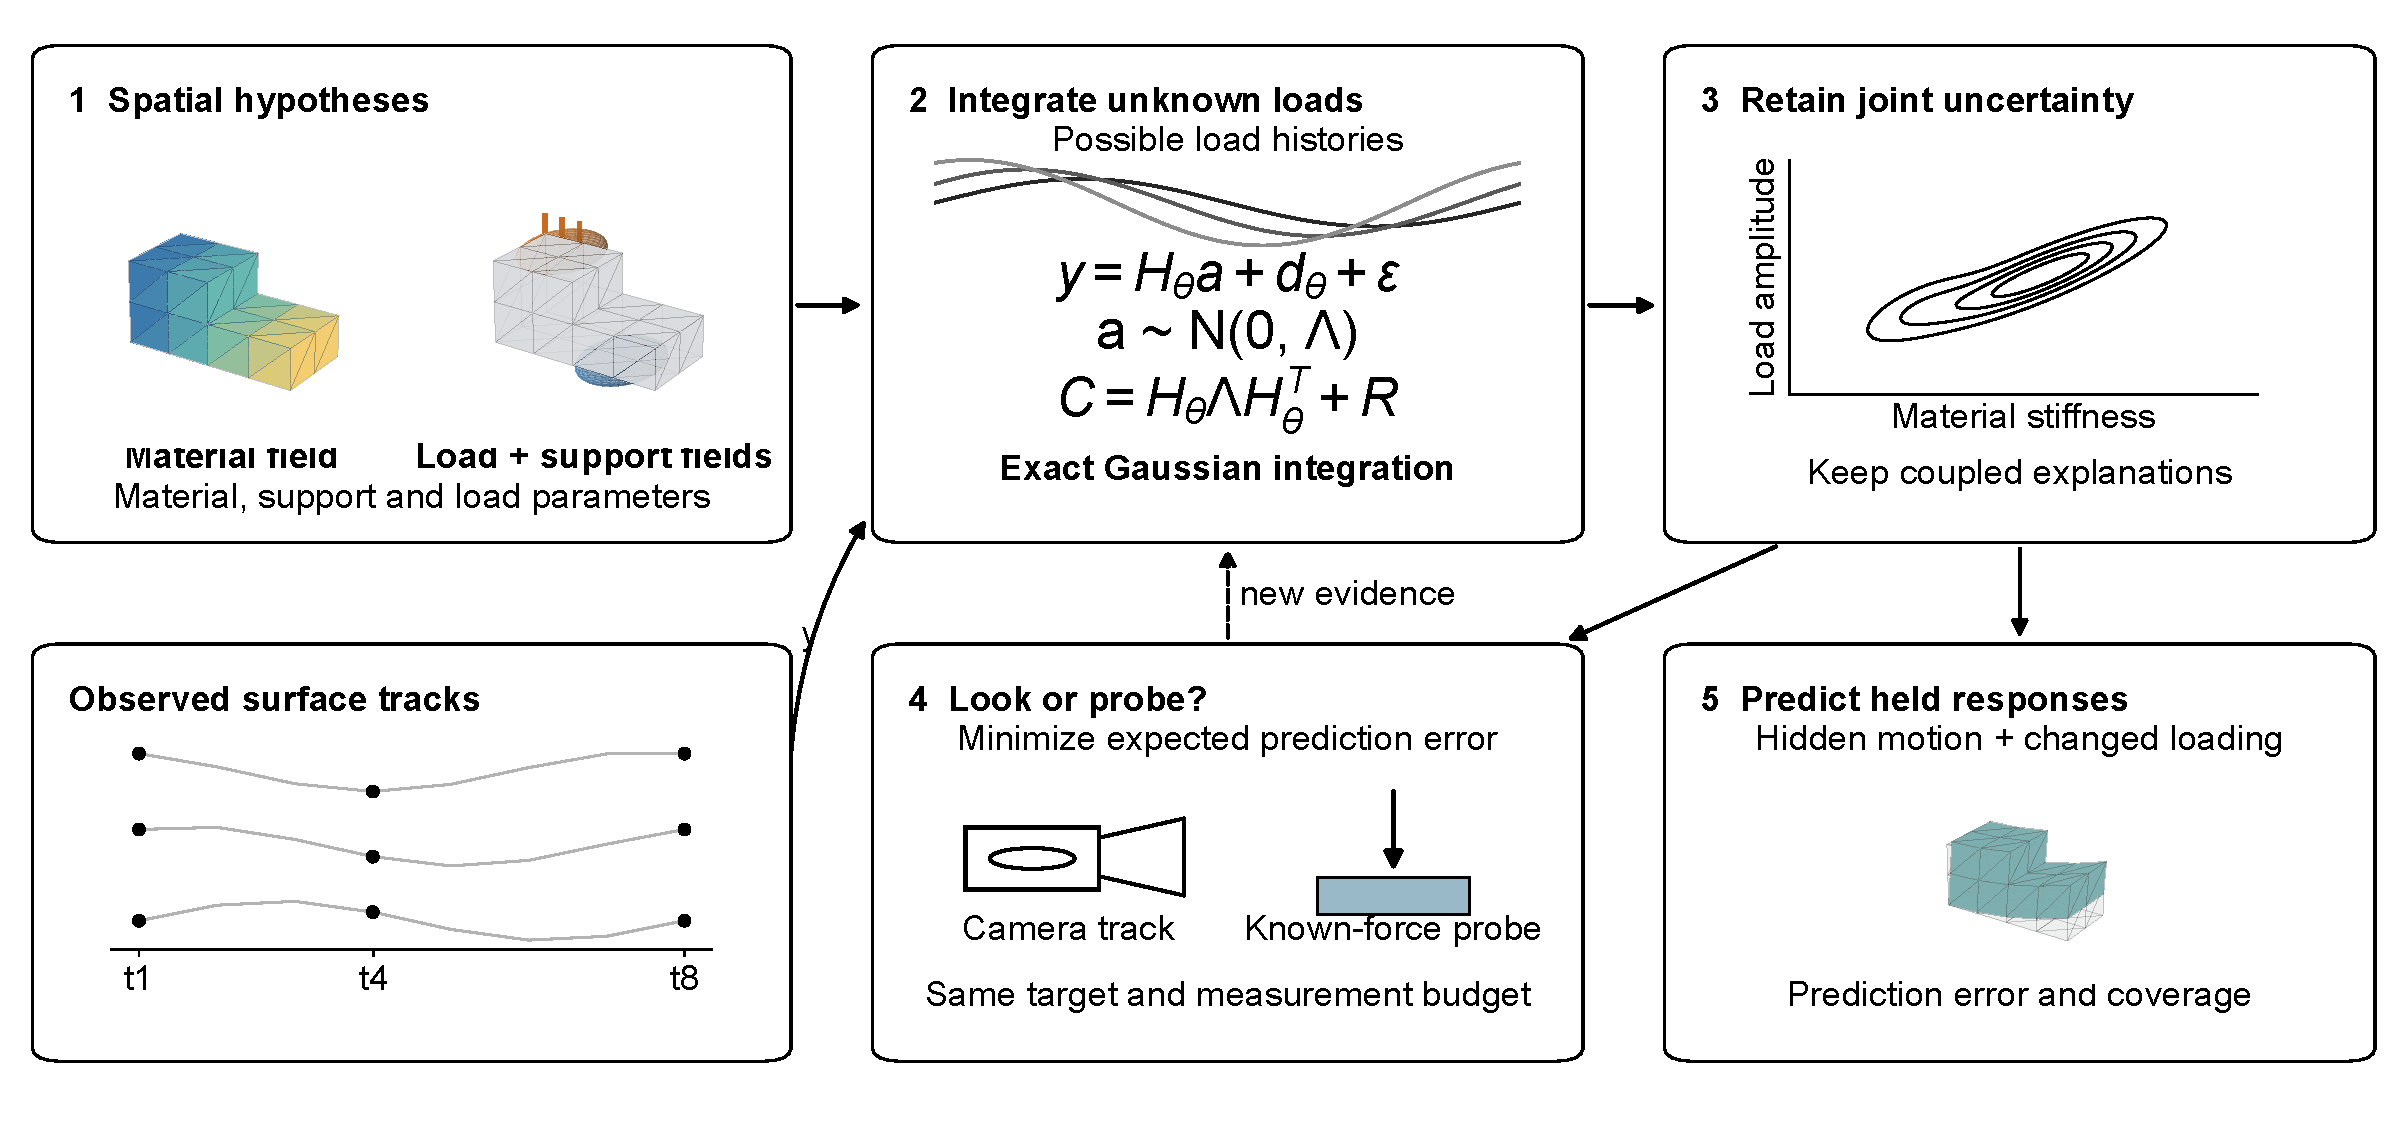
\includegraphics[width=.98\textwidth]{figures/method.pdf}
\caption{\textbf{Joint identification, with mechanics as the forward model.} Sparse projected movement constrains separate material and interaction fields. Gaussian load amplitudes are integrated conditionally, producing correlated physical explanations. A fixed predictive target guides either a camera-track measurement or a calibrated reset probe. The schematic distinguishes these operations from the known-geometry assumptions of the evaluated reference.}
\label{fig:method}
\end{figure*}
Let $X$ denote material coordinates and $u_t$ displacement. Reference geometry, camera projections and track correspondences are supplied. We use incremental, gravity-free quasistatic response about an unloaded configuration, with fixed Poisson ratio. This deliberately controlled setting permits the inverse calculation to be checked independently of geometry recovery, tracking errors and nonlinear contact.

\paragraph{Material field.}
Two fixed Gaussian features form a normalized partition,
\begin{align}
\bar\phi_j(X)=\frac{\exp[-\tfrac12\|X-c_j\|^2_{S^{-1}}]}{\sum_l\exp[-\tfrac12\|X-c_l\|^2_{S^{-1}}]},
\\
E(X)=\exp\{m_0+m_1\chi(X)\},
\end{align}
where $\chi$ is the volume-centered difference of the two features. Thus $E>0$, and $m_0,m_1$ control mean log modulus and spatial contrast. Centers and widths are fixed in this experiment. This is a low-dimensional spatial family in 3D, not arbitrary heterogeneous-material discovery.

\paragraph{Support and unknown traction.}
For a surface $\Gamma$, a Gaussian gate is normalized by its surface integral,
\begin{equation}
 w(X;c)=\frac{\exp[-(X_x-c)^2/(2\ell^2)]}
 {\int_\Gamma\exp[-(X'_x-c)^2/(2\ell^2)]\,dA'}.
\end{equation}
The support energy is $\tfrac12k_b\int_{\Gamma_b}w_b\|u\|^2dA$. The implementation uses declared nodal lumping of the surface quadrature. Two unknown traction modes act downward on the top and laterally on a side, with a shared inferred longitudinal center $c_f$. Each mode has unit-integral spatial weights and a time-dependent scalar amplitude in newtons. Signed amplitudes describe applied traction; neither this prior nor a bilateral support spring implements unilateral contact.

The nonlinear physical coordinates are
\begin{equation}
\theta=(\log E_0,m_1,c_b,\log k_b,c_f).
\end{equation}
The finite-element equilibrium and projected observation maps are
\begin{equation}
 K(\theta)u_t=B(\theta)a_t+f_t^{\rm known},\qquad
 y=H_\theta a+d_\theta+\epsilon.
\label{eq:forward}
\end{equation}
Here $a$ stacks two modes at eight loading times; $H_\theta$ includes the stiffness solve and known camera projection. The support removes rigid modes without a hidden numerical pin. Surface normalization ensures that refining the mesh does not change the intended total applied force.

\paragraph{Gaussian uncertainty is a separate role.}
The spatial kernels above locate physical properties and interactions. The load prior $a\sim\mathcal N(0,\Lambda)$ instead describes uncertainty over temporal amplitudes, with a Mat\'ern-$3/2$ covariance. Neither is the same as an appearance Gaussian used in rendering. Maintaining these roles avoids interpreting splat opacity as mass or confusing a footprint width with posterior uncertainty.

\section{Inference with Analytically Marginalized Loads}
For each field hypothesis, observations satisfy a linear-Gaussian model with covariance $R$. Eliminating $a$ gives
\begin{align}
 C_\theta&=R+H_\theta\Lambda H_\theta^\top,\\
 p(y\mid\theta)&=\mathcal N(y;d_\theta,C_\theta).
\label{eq:marginal}
\end{align}
The marginal objective includes both the quadratic residual and $\log|C_\theta|$. Both change when material or interaction geometry changes. Dropping the determinant does not preserve this probabilistic model.

The conditional force distribution is
\begin{align}
 m_\theta&=\Lambda H_\theta^\top C_\theta^{-1}(y-d_\theta),\\
 S_\theta&=\Lambda-\Lambda H_\theta^\top C_\theta^{-1}H_\theta\Lambda.
\end{align}
The finite implementation uses Cholesky solves and a Joseph-form covariance update to avoid subtractive loss of positive definiteness. We retain dependence between $\theta$ and $a$:
\begin{equation}
 \Var[a\mid y]=\E_\theta[S_\theta]+\Var_\theta[m_\theta].
\label{eq:totalcov}
\end{equation}
Reporting only $S_{\hat\theta}$ would condition away ambiguity in the fitted physical explanation.

\paragraph{Reference and continuous inference.}
A predeclared $5^5=3125$-hypothesis dictionary gives weights $w_h\propto p(y\mid\theta_h)p(\theta_h)$ and exact Gaussian force conditionals. ``Exact'' refers to this finite model, not a continuous parameter posterior or the real object. Continuous inference uses a uniform prior in the declared five coordinates and adaptive tempered sequential Monte Carlo~\cite{delmoral2006smc}. Conditional load integration is unchanged. Reflected Metropolis moves remain within the bounds; all invalid likelihoods are retained as zero-weight/rejected states. Separate seeds and particle counts audit Monte Carlo sensitivity. The discrete prior assigns mass to endpoints, so finite/continuous differences are not solely integration error. Continuous inference reevaluates the recorded actions selected by the finite-dictionary planner; it is not a separately evaluated continuous acquisition policy. Its conditional covariance uses a symmetrized Gaussian subtraction formula, independently checked in numerical tests.

\paragraph{Uncertain force scale.}
An assumed force magnitude can supply apparent stiffness information. We therefore also infer a latent amplitude scale $\tau$ with $\Lambda_\tau=\tau^2\Lambda$. Five equally weighted log-spaced scales from $0.5$ to $2$ define a separately frozen finite mixture,
\begin{equation}
p(\theta,\tau\mid y)\propto p(y\mid\theta,\tau)p(\theta)p(\tau).
\end{equation}
Conditional integration remains Gaussian; material--scale dependence remains in the outer mixture. A broader single Gaussian with the same prior force variance controls for merely increasing uncertainty. An oracle receives the true scale, while a fixed nominal model does not. This finite hyperprior exposes sensitivity to absolute force calibration. A separately frozen follow-up additionally mixes three temporal correlation lengths, giving $\Lambda_{\tau,\ell_f}=\tau^2\Lambda_{\ell_f}$. It tests a specified temporal-prior failure; the finite choices are not an unrestricted force-prior estimator.

\paragraph{What marginalization changes.}
With fixed force mapping and discrepancy, our earlier trajectory experiment verified equivalence between profiled joint and marginalized stationary points. That simplification does not generally apply here. At a given hypothesis, the joint posterior density at its conditional force mode differs from the marginalized density by $-\tfrac12\log|S_\theta|$ plus a constant. Our joint-MAP and marginal-MAP controls therefore estimate different summaries; any difference is not advertised as a pure optimizer speedup. A direct Gaussian conditioning identity is the numerical correctness control.

\paragraph{Relation to nonlinear image fitting.}
In a nonlinear trajectory formulation, a residual $r(z)=G(z)a+\eta$ still permits exact force elimination conditional on the trajectory/material state $z$. Rendering and the remaining posterior can be nonlinear and approximate. Our earlier cube experiment implemented that distinction. The new cohort uses affine projected tracks precisely to make the conditional likelihood and finite posterior auditable; it does not claim that Eq.~\eqref{eq:marginal} is the exact RGB likelihood of a general Gaussian renderer.

\section{Observability and Measurement Selection}
\paragraph{A physical ambiguity.}
When $K$ scales with elastic and support stiffness, replacing $(E,k_b,a)$ by $(cE,ck_b,ca)$ leaves Eq.~\eqref{eq:forward}'s unknown-load displacement unchanged. No additional camera can break this conditional observation-map symmetry. A fixed load prior may prefer one scale, but that preference is prior information. With latent amplitude scale, corresponding hypotheses satisfy
\begin{equation}
H_{\theta'}=H_\theta/c,\quad \Lambda_{\tau'}=c^2\Lambda_\tau
\quad\Longrightarrow\quad C_{\theta',\tau'}=C_{\theta,\tau}.
\end{equation}
Their force-marginalized likelihood components are identical for every track observation; this is not a statement that the complete parameter marginals have equal mass under bounded priors. The teaser verifies two such components within the declared dictionaries. A known reset load does not co-scale, so its response changes and can distinguish them.

\paragraph{One fixed prediction target.}
Let $q=T_\theta a+b_\theta$ concatenate unobserved original-load displacements and reset responses under four new known loads. None of its original-motion points is acquired; its reset loads differ from the acquisition probes. Both groups contain 192 scalar coordinates, giving equal group weight. The squared-error Bayes risk is
\begin{equation}
 \mathcal R(D)=\frac{1}{384}\sum_j\Var(q_j\mid D).
\end{equation}
This is a predictive objective, not a requirement to recover every material coefficient.

\paragraph{Camera and probe updates.}
A scalar action produces $y_s=h_{s,\theta}a+d_{s,\theta}+e_s$. A camera action has $d=0$ and observes another projection of the original experiment. A calibrated probe uses a reset object, so $h=0$ and $d$ is its known-load response. Both update hypothesis weights. A camera also updates conditional original forces; a probe leaves those conditionals unchanged while reweighting their mixture. The candidate score is
\begin{equation}
 s^*=\arg\min_s\E_{y_s\mid D}\big[\mathcal R(D\cup\{s,y_s\})\big].
\end{equation}
We estimate this expectation using 128 predictive draws with common random numbers and audit predeclared decisions at 1024. Four greedy acquisitions are compared against a development-selected fixed mixed schedule, fixed camera-only and probe-only schedules, and random selection without replacement. Each action costs one scalar track measurement. Reset, execution time, force calibration error and robot safety are outside this reference cost model. Original loading is replayable; acquiring an earlier time is not online travel into the past.

\section{Experiments}
\paragraph{Scenes and observations.}
The block and stepped block occupy a $120\times60\times60$\,mm bounding box. The inference meshes contain 225 and 185 nodes. Volume-geometric mean modulus ranges from 8 to 32\,kPa, log contrast from $-0.8$ to $0.8$, support center from $-25$ to $25$\,mm, support stiffness from 4 to 16\,kN/m, and load center from $-40$ to $40$\,mm. There are 24 initial scalar observations: four front-surface points, two orthographic components and three loading times. Additional back-surface tracks use an oblique camera whose measured direction is orthogonal to its viewing ray. A ray--triangle audit on all deformed load and probe states verifies visibility, including an occluded-marker negative control. Noise is 0.02\,mm; unknown load standard deviation and calibrated probe magnitude are 0.08\,N. These precise known-correspondence measurements are an idealized identification setting, not a claim about real tracking accuracy.

\paragraph{Independent populations.}
The primary matched finite-prior cohort has 64 cases per geometry. Three further populations each have 32 cases per geometry: continuous parameters on the same mesh; continuous parameters on a finer $12\times6\times6$ cell mesh; and a shorter true force correlation length, leaving inference unchanged. No final case supplies model selection. Twelve separate development cases per geometry choose fixed schedules. A further 128 fresh surface-track cases test the hierarchical force-scale model, with four fixed views or four fixed probes applied as separate branches from the same initial evidence. A subsequent 64-case follow-up tests additional temporal-prior uncertainty on fresh short-correlation force histories; its motivation and conditional stress-test scope are reported separately. Model sources, priors, seeds, targets and budgets are hashed before final evaluation.

\paragraph{Controls and metrics.}
Point-estimate controls retain either the marginal-MAP or joint-MAP hypothesis. Representation controls remove material contrast or fix interaction geometry/stiffness. A moment-independence control retains the material marginal and force first two moments but removes their dependence; it is not the full product of two exact mixture distributions. We report mean per-case coordinate RMSE, material-field relative error, force amplitude error and a normalized longitudinal load-basis profile proxy, and equal-tail 90\% marginal coverage. Prediction coverage uses 24 fixed coordinates, not an entire-path guarantee. Case-bootstrap comparisons are paired across the two fixed geometries and do not establish generalization over a population of shapes.

\paragraph{Numerical qualification.}
Unit tests verify stiffness symmetry, rigid modes, force normalization, gradients, CPU/GPU agreement, Gaussian identities, sequential/batch updates and inference input separation. A separate 2.5-fold scaling test preserves all tested camera projections within $4.04\times10^{-18}$\,m, while the same calibrated probe gives a response ratio of 0.4. Stronger supports were selected before final testing to avoid almost rigid excitation. Representative corner tests give maximum principal strain 2.02\%/2.61\% and median nonrigid/total RMS 19.5\%/28.2\% for block/step. Gaussian tails are not truncated. Mesh sensitivity remains material: representative $8\to16$ refinement differences range from 0.027 to 0.209\,mm. The finer-mesh population therefore tests mismatch rather than assuming the coarse generator is physically exact.

\section{Results}
\begin{table}[t]
\centering\small
\caption{\textbf{Joint identification and added evidence.} Matched finite-prior cohort; means of case-level errors after four scalar measurements. Hidden and new-load entries are coordinate RMSE. All policies use the same initial observations and fixed target.}
\label{tab:acquisition}
\begin{tabular}{lrrrr}\toprule
Policy & Hidden & New load & Material & Force\\
 & mm & mm & rel. & N\\\midrule
Initial & 0.076 & 0.024 & 0.451 & 0.042\\
Active & 0.045 & 0.014 & 0.347 & 0.030\\
Fixed & 0.057 & 0.012 & 0.322 & 0.033\\
Fixed View & 0.050 & 0.022 & 0.421 & 0.032\\
Fixed Probe & 0.074 & 0.010 & 0.277 & 0.040\\
Random & 0.059 & 0.014 & 0.343 & 0.034\\
\bottomrule\end{tabular}
\end{table}
\begin{figure*}[!t]
\centering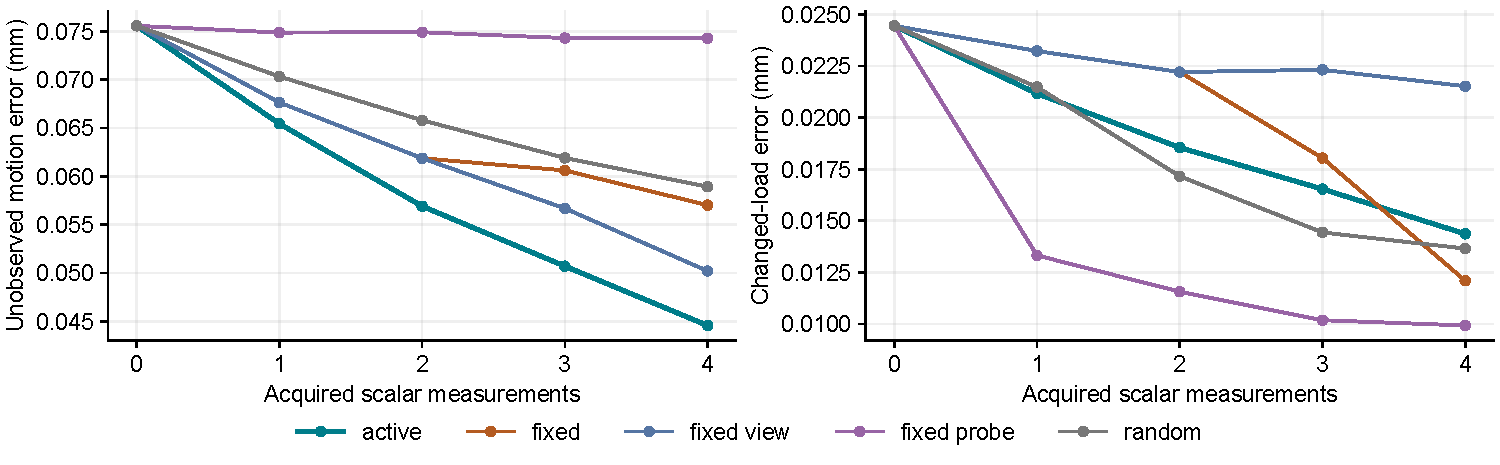
\includegraphics[width=.98\textwidth]{figures/acquisition-prediction.pdf}
\caption{\textbf{Prediction targets favor different measurements.} Complete matched-cohort hidden-motion and new-load errors against acquisition count. Fixed mixed, camera-only and probe-only schedules were selected on separate development cases. Curves retain all cases and do not imply that every scene benefits from adaptive selection.}
\label{fig:acquisition}
\end{figure*}
\begin{figure*}[!t]
\centering\IfFileExists{figures/hierarchy-summary.pdf}{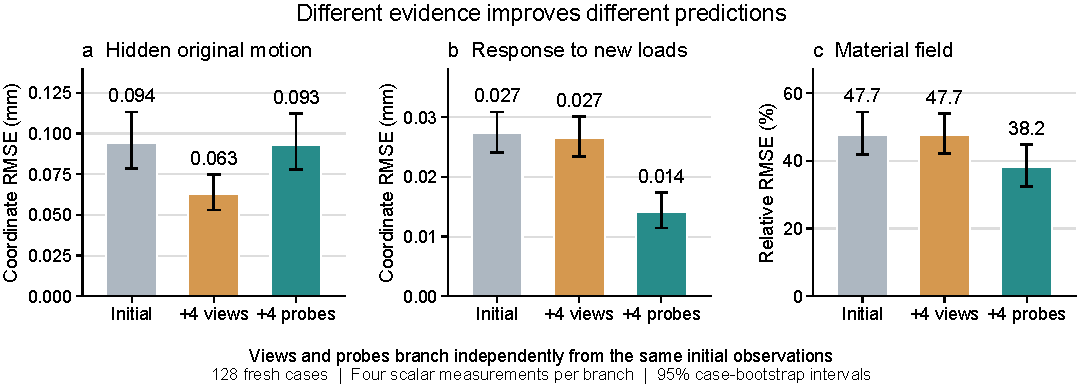
\includegraphics[width=.98\textwidth]{figures/hierarchy-summary.pdf}}{\fbox{Hierarchical study running}}
\caption{\textbf{Views and probes resolve different uncertainties.} Fresh force-scale cohort; each four-measurement branch starts from the same initial data. Views reveal hidden motion; known loads test the material/support response without relying on the original unknown force. Intervals show uncertainty in cohort mean errors.}
\label{fig:hierarchy}
\end{figure*}

\begin{figure*}[!t]
\centering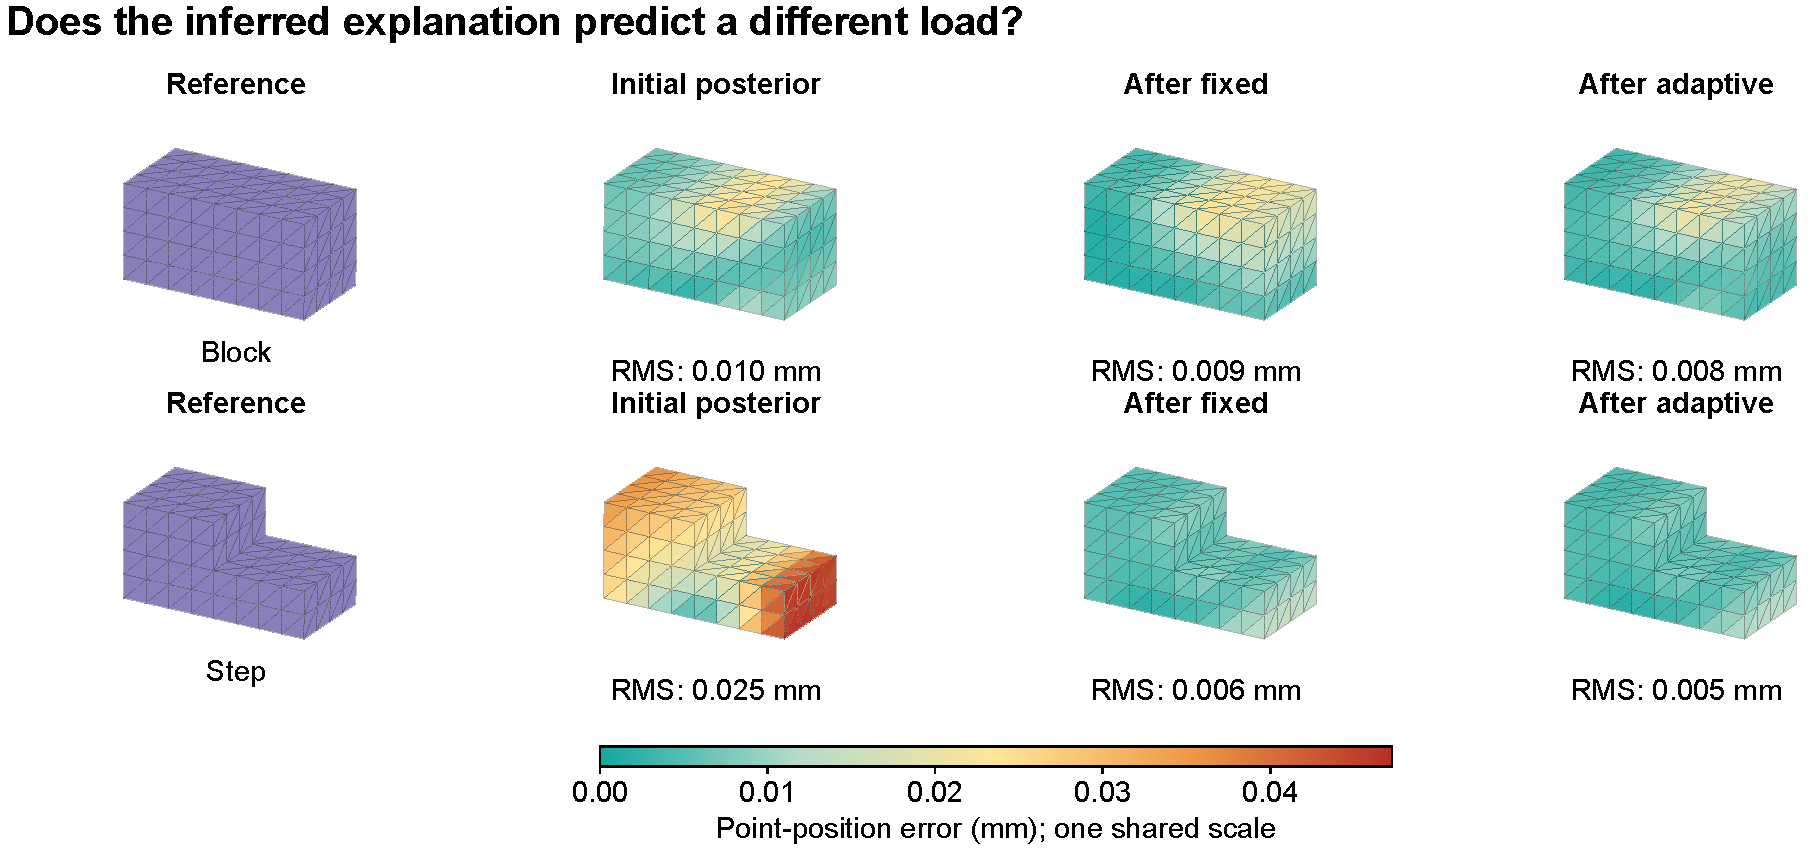
\includegraphics[width=.98\textwidth]{figures/changed-load-comparison.pdf}
\caption{\textbf{A new load tests the inferred explanation.} Predeclared case zero in each geometry, under a held 0.08\,N load at $x=20$\,mm. Shared color scales show point-position errors; headers report volume-weighted nodal errors, a different metric from the coordinate tables. These fixed examples include improvement and persistent error. Geometry is shown at true scale; the panels are not photorealistic RGB predictions.}
\label{fig:qualitative}
\end{figure*}
\begin{figure}[!t]
\centering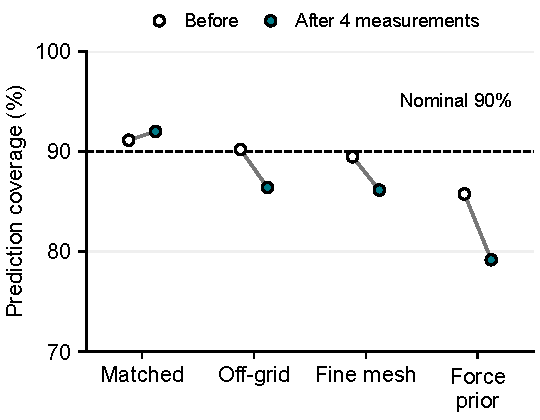
\includegraphics[width=\linewidth]{figures/coverage-prediction.pdf}
\caption{\textbf{Uncertainty under mismatch.} Each segment joins initial and post-acquisition prediction coverage. The dashed line is nominal 90\%; the percentage axis is zoomed. Dictionary exactness does not guarantee coverage for continuous, mesh-mismatched or force-prior-mismatched truth.}
\label{fig:coverage}
\end{figure}

\paragraph{Prediction after additional evidence.}
Across 128 matched surface-track cases, four adaptive scalar measurements change combined coordinate RMSE from 0.0578 to 0.0340\,mm. The development-selected fixed mixed schedule gives 0.0423\,mm, camera-only gives 0.0403\,mm, and random selection gives 0.0438\,mm. The paired adaptive-minus-fixed difference is -0.0083\,mm, with 95\% case-bootstrap interval [-0.0110,-0.0058]. Against fixed camera-only, the paired difference is -0.0063\,mm [-0.0083,-0.0043]. The adaptive policy selects 439 camera and 73 probe measurements across 512 decisions. These are complete-cohort comparisons under the declared equal-weight target, not selection of favorable objects.

\paragraph{Different measurements serve different predictions.}
Adaptive selection gives hidden-motion/new-load errors 0.0446/0.0144\,mm. The probe-only policy gives 0.0743/0.0099\,mm; camera-only gives 0.0502/0.0215\,mm. A policy can therefore be useful for changed interactions without being best for reconstructing the original load sequence. The adaptive policy is worse than fixed mixed for new-load and material error; its advantage concerns the combined target. The shared objective makes this tradeoff explicit (Fig.~\ref{fig:acquisition}).

\paragraph{Unknown force magnitude and calibrated evidence.}
The independent 128-case scale-mixture study tests whether apparent material certainty is supplied by the force prior. Under the hierarchical model, four calibrated probes change new-load error from 0.0274 to 0.0141\,mm and material relative error from 0.477 to 0.382. Four views instead give hidden-motion error 0.0626\,mm, compared with 0.0939\,mm initially. Mean log-stiffness/log-force-scale posterior correlation is 0.346 initially and 0.181 after probes. These branches start from the same initial evidence.

After probes, hierarchical force intervals have 88.8\% coverage and 0.158\,N mean width; fixed nominal intervals have 81.9\% coverage and 0.134\,N width. The variance-matched broader Gaussian gives 86.6\% coverage and 0.163\,N width. The hierarchy is thus compared with an explicit wider-prior control, rather than interpreting width alone as calibrated identification.

\paragraph{Dependence, continuous inference and mismatch.}
After adaptive evidence, retaining joint dependence gives mean prediction-interval width 0.0717\,mm versus 0.0863\,mm for the moment-independence control, with coverages 92.0\%/93.9\%. Hidden-motion errors are nearly equal (0.0446/0.0449\,mm); the benefit is interval efficiency, not a large mean-prediction gain. The supplement retains all point and representation controls. On 64 continuous-prior cases, continuous inference gives post-adaptive RMSE 0.0294\,mm versus 0.0350\,mm for fixed mixed measurements. The posthoc paired 95\% interval for their difference is [-0.0088,-0.0027]\,mm. Prediction/force 90\% coverages are 89.7\%/91.2\%. All 192 main fits and 96 seed/particle diagnostics completed; 2 of 144 descriptive sensitivity comparisons exceed the declared thresholds. These checks do not certify convergence. Actions were selected by the finite planner, and the continuous and finite priors differ.

For the finite-dictionary estimator, matched adaptive prediction intervals cover 92.0\% of evaluated coordinates at nominal 90\%. Coverage becomes 86.4\% for continuous parameters, 86.1\% for finer-mesh truth, and 79.2\% for the shorter-correlation force prior. These tests distinguish conditional numerical exactness from robustness to a different generator.

\paragraph{Actual spatial force distributions.}
A separately declared posthoc diagnostic integrates traction errors over the loaded surfaces and all loading times. Joint posterior-mean traction RMSE changes from 10.15 to 7.18\,Pa after adaptive evidence; fixed mixed measurements give 8.04\,Pa. Joint and product-marginal mean fields are nearly identical on this endpoint; the force-field improvement comes from additional evidence. This field metric complements the original one-dimensional load-basis proxy.

\paragraph{A targeted temporal-prior repair.}
On 64 fresh conditional stress cases, mixing correlation length as well as amplitude reduces hidden-motion error after four fixed views from 0.1170 to 0.1007\,mm. Force 90\% coverage rises from 72.4\% to 83.9\%, while width rises from 0.138 to 0.177\,N. The known-covariance oracle gives 91.7\% coverage. Material relative error worsens from 0.476 to 0.506; improved force interpolation does not establish better material recovery. This posthoc follow-up retains the original mismatch failures.

\paragraph{Forward-model discretization.}
In the separate 32-case interior-sensor reference, refining the inverse model changes post-adaptive prediction coverage from 76.7\% to 87.2\%. Overall RMSE changes modestly, 0.0415 to 0.0403\,mm; its paired interval includes zero improvement. Numerical accuracy of the forward model therefore matters for physical uncertainty as well as response error.


\section{Connection to Existing Rendering and Physical Benchmarks}
The previous platform provides supporting evidence about forward models and the limits of visual agreement. These experiments use different adapters and are not comparisons of the newly marginalized posterior. Across six simulated contact/interaction families and 24 material worlds, the learned continuum model has 1.97\,mm motion RMS versus 10.80 and 11.27\,mm for adapted PhysTwin and Spring-Gaus; a matched analytic continuum control achieves 1.84\,mm. Known boundaries and a continuum-generated reference favor this comparison's model family. It does not show that Bayesian identification outperforms those methods.

On eight released real PhysTwin continuations, the prior neural equilibrium adapter has 39.01\,mm tracking error versus 21.14\,mm for released PhysTwin. Shared-appearance PSNR is 16.13 versus 17.66\,dB. Two geometry-qualified changed-interaction pairs favor the frozen adapter in mean, 39.16 versus 44.63\,mm, but the individual outcomes are mixed. On 40 fresh SoftVT episodes~\cite{jing2026softvt}, the separate slip-aware predictor reduces coordinate error from 18.932 to 17.865\,mm (5.64\%); its shape error is unchanged, so the gain concerns placement. These public recordings do not provide the spatial force/material labels or calibrated reset interventions needed to validate the new recovery claims. The complete historical cohorts, contacts, rendering comparisons and negative PIDG~\cite{hong2026pidg} forecast remain archived; none is promoted into a joint-field result.

The original sparse-RGB cube study is a closer inference predecessor. Under a fixed spatial force profile, exact amplitude elimination and joint optimization give similar reconstruction errors, without consistent speed superiority. Its local trajectory posterior is not generally calibrated. The new work changes the scientific question to spatial hypotheses and action selection, and uses a linear observation reference to expose inference error separately from rendering error.

\section{Discussion and Limits}
The forward solver is a means to evaluate competing physical explanations. The distinctive evaluated object is their posterior predictive distribution and its response to new evidence. Analytical elimination removes a tractable nuisance block; it neither creates information nor makes spatial material and load fields uniquely identifiable. A fixed prior can regularize an ambiguity without resolving it experimentally.

Our current spatial family varies longitudinally through five parameters. Geometry, cameras, correspondences, Poisson ratio and kernel widths are known. The new reference contains no unknown contact graph, friction, impact, damping or inertia. Continuous SMC is approximate, and the scalar camera/probe cost abstraction omits hardware constraints. General RGB reconstruction, large nonlinear deformation and real calibrated probing remain extensions, not completed capabilities. The method can be coupled to richer mechanics through conditional force elimination, but that remaining nonlinear posterior requires its own numerical and calibration checks.

\paragraph{Conclusion.}
Jointly representing material and interaction uncertainty makes the distinction between observed motion and physical identification explicit. Conditional load marginalization supplies a tractable inference component, while new-view and calibrated-load measurements provide different information. The controlled reference, continuous extension and mismatch audits establish the scope of the resulting predictions without treating a plausible render or a successful mechanics solve as proof of physical truth.

\clearpage
{\small\bibliographystyle{ieeenat_fullname}\bibliography{references}}
\paragraph{LLM usage declaration.} Language-model coding assistants assisted implementation, experiment orchestration, literature organization and manuscript preparation. Numerical claims are tied to saved outputs and executable checks. Author review and responsibility remain necessary before submission.
\end{document}
